\documentclass[a4paper,10pt]{article}

\usepackage{ctex} % For Chinese text support
\usepackage{geometry} % For page dimensions
\usepackage{graphicx} % For including images
\usepackage{marginnote} % For margin notes (side notes)
\usepackage{fancyhdr} % For custom headers and footers
\usepackage{lipsum} % For generating filler text (optional)
\usepackage{fontspec}
\usepackage[dvipsnames]{xcolor}
\usepackage{titlesec}
\usepackage{ragged2e}
\usepackage{ctex} % Chinese fonts
\usepackage{framed}


% Set a font that includes the solid square symbol
\setmainfont{Arial}

% Set the page margins
\geometry{
    left=2.5cm, 
    right=2.5cm, 
    top=2.5cm, 
    bottom=2.5cm
}
\setlength\parindent{24pt}


% Define a command for rotated side notes
\newcommand{\rotatedsidenote}[1]{%
  \marginnote{\rotatebox{270}{\raggedright\small#1}}%
}


% Setup fancyhdr for headers and footers
\pagestyle{fancy}
\fancyhf{} % Clear all header and footer fields
\fancyhead[L]{\small ■ \heiti 大地巡旅} % Left header
\fancyhead[C]{\hspace{11cm} \small ■ TERRA: A JOURNEY} % Center header
\renewcommand{\headrulewidth}{0pt} % Remove the header line

% Redefine the plain page style to use the same header/footer as fancy
\fancypagestyle{plain}{
  \fancyhf{} % Clear all header and footer fields
  \fancyhead[L]{\small ■ \heiti 大地巡旅} % Left header
  \fancyhead[C]{\hspace{11cm} \small ■ TERRA: A JOURNEY} % Center header
  \renewcommand{\headrulewidth}{0pt} % Remove the header line
}


% Set Epigraph style
\renewenvironment{leftbar}[1][\hsize]
{%
    \def\FrameCommand
    {%
        {\color{SpringGreen}\vrule width 3pt}%
        \hspace{8pt}%must no space.
    }%
    \MakeFramed{\hsize#1\advance\hsize-\width\FrameRestore}%
}
{\endMakeFramed}

%%%%%%%%%%%%%%%%%%%%%%%%%%%%%%%%%%%%%%%%%%%%%%

\begin{document}


\section*{\textcolor{SpringGreen}{■ } \heiti 明日方舟}

\noindent
\begin{minipage}[t]{0.7\textwidth} % Left column (70% of the width)
    \noindent
    \setlength\parindent{20pt} \#记录生活 \ 请问玩游戏的玩家们有没有看过日本所谓的明日方舟官方世界观设定集，《大地巡游》。

    \subsection*{\hspace{20pt}有毒的世界观}
    \setlength\parindent{20pt} 关于源石，书中的设定说是矿物结晶，但其实非也，根据后面定义的源石技艺，也就是人类怎么用它的六大法术体系来反推断，这个源石其实是指人类的智力，体力和思维能力。

    \subsection*{\hspace{20pt}有毒的游戏}
    \setlength\parindent{20pt} 所以书中构造的从源石天灾大气微粒到人类得的传染病，所谓的矿石病，根本经不起简单的逻辑推敲，如果非得说有这种病，那就是说人类的智力体力和思维能力成了人人可怕的致死的在死后还可以飞速传染的传染病。

% textbf{}无法加粗中文部分
\begin{leftbar}
    \kaishu \small
    这不是反教育，反人性创造力的世界观是什么？从高中一直到大学，学生们若最美好的时光都用来玩这个游戏了，他的成绩会怎么样？他如何走向社会？
    \\
    {\hbox{}\nobreak\hfill——咖啡雨，编辑于2024-06-12} 
\end{leftbar}

\section*{\textcolor{SpringGreen}{■ } \heiti 虚构的荒谬的世界观}
%    \setlength\parindent{22pt} 这样一个虚构的荒谬的世界观的游戏里里，玩家们每天因公司游戏设置强行都要上去操弄最少10分钟半个小时的，这个游戏因借用二次元形象设计还生产了很多的衍生商品，吸引了众多二次元粉丝参与游戏，游戏商家也在游戏中赚取了玩家们的金钱。\par
    \setlength\parindent{20pt} 这里面有不少是初中生吧，或者高中生然后延续到大学，如果游戏作为解压，仅仅是游戏可以随时放下的，那可以理解，如果这样一种虚假的源石本质和技艺在逻辑上根本不成立的虚构，并由此引发一个恐慌和冲突的塔防游戏世界，长期沉迷其中导致玩家大脑结构的损坏和错误世界观的根植，那么游戏的设计者，世界观设定集的作者以及商家，纯粹是为了谋利，根本没有想到在他们牟利的同时，让这个社会的年轻人失去了什么，其心可诛。这已经不是伤心的层次了。

    \begin{center}
    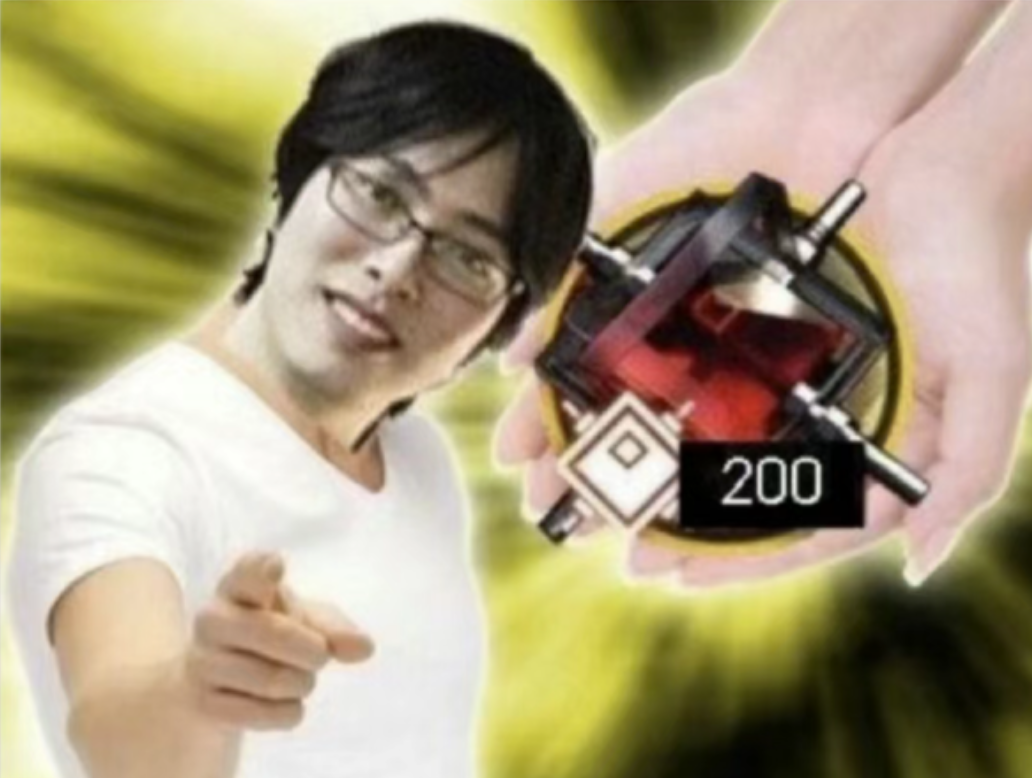
\includegraphics[width=0.9\linewidth]{海猫合成玉.png} % Replace with your image file
    \\
    \justifying \small ■ \heiti 图例
    \end{center}


\end{minipage}%
\hfill
\begin{minipage}[t]{0.25\textwidth} % Right column (25% of the width)
    \rotatedsidenote{■ \thepage \hspace{15cm} CHAPTER 42 Arknights Dank Memes / 42.1 Coffe Rain}
{\heiti
    \textcolor{SpringGreen}{■ } \textbf{源石技艺适应性}\\
    \hspace*{8pt} 缺失\\
    \\
    \textcolor{SpringGreen}{■ } \textbf{眼神}\\
    \hspace*{8pt} 呆滞\\
    \\

    \vspace{0.4cm} % Add some space before the image

    \begin{center}
    
\includegraphics[width=\linewidth]{海猫种水稻.png} % Replace with your image file
    \justifying \small 图例
    \end{center}
    }
    

\end{minipage}

\end{document}
